\chapter{Background}
\label{ch:background}
The theoretically limitless resources of the cloud and the growing popularity of modern web applications have created a need for distributed systems on a scale which has never been seen before. Problems of scale are no longer confined to the supercomputing community. In this section, we describe the cloud ecosystem, the challenges surrounding it, and the tools to manage it.

\section{The ``Cloud''}
The term ``cloud computing'' is used to describe applications or resources which are managed by an external provider and accessed over a network. In the case of this work, when we refer to cloud services, we are specifically referring to services which offer computing resources as their primary product.

\section{Types of Scaling}
Scaling in the cloud can be as simple as the push of a button. It is important to understand the different ways an application can scale in this environment, as well as the trade-offs associated with each method.

There are two types of scaling, horizontal and vertical \cite{allspaw2008art}. Vertical scaling refers to increasing the size of the hardware which a system runs on. A simple example of vertical scaling would be adding more RAM to a machine. In cloud computing, vertical scaling manifests itself in moving applications onto larger virtual machines. Horizontal scaling is the addition of more machines to a computing cluster. Purchasing of more servers or launching more VMs are the two most common examples of horizontal scaling. Although the term ``scaling up'' seems like it would apply to vertical scaling, it is most commonly used in reference to horizontal scaling.

Applications often avoid scaling horizontally for as long as possible because the separation of an application onto more than a single machine introduces another layer of complexity and need for coordination between machines. However, a single machine can only scale with demand for so long. Many large modern web services operate on hundreds of machines. Horizontal scaling is also much more elastic than vertical scaling; it is much easier to add and remove many VMs quickly than it is to change the capacity of existing VMs. For this reason, CRAFTS focuses on horizontal scaling. Unless stated otherwise, it can be assumed that any reference to scaling in this paper refers to horizontal scaling.

\begin{figure}
\centering
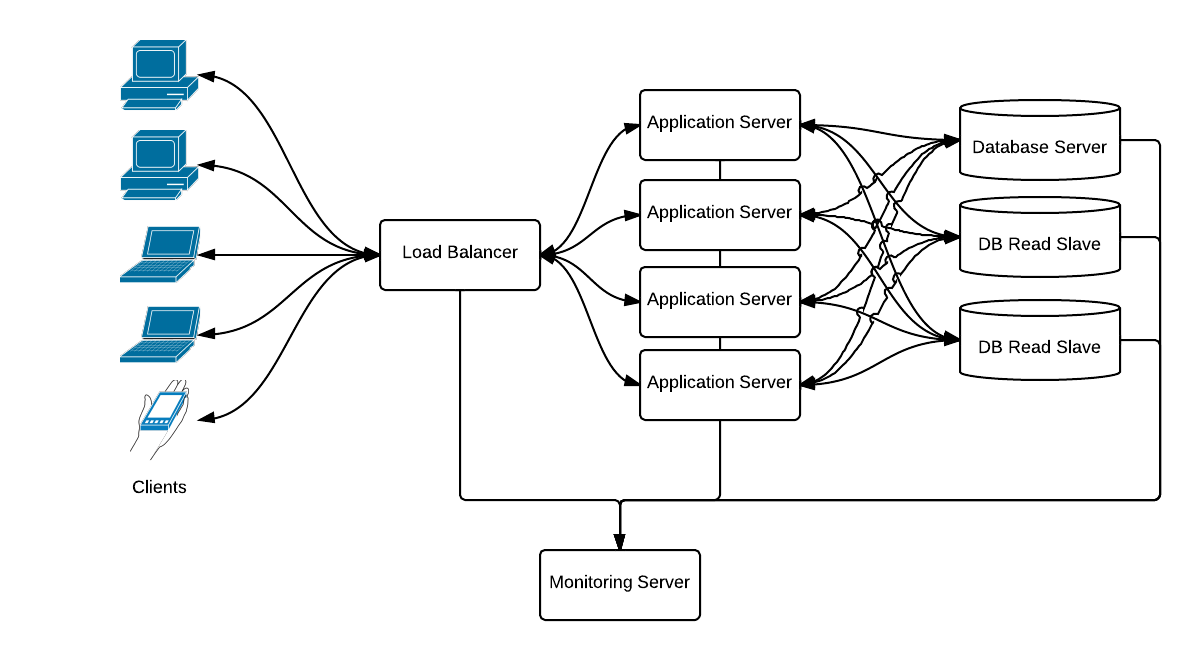
\includegraphics[width=\textwidth]{diagrams/highavailability.png}
\caption{Example architecture of a high availability application.}
\label{fig:highavailability}
\end{figure}

\section{High Availability Applications}
Not every system needs to be constantly scaled up and down. Applications that are not required to produce results in real-time can be scaled in order to produce a result in a specific amount of time. MapReduce \cite{dean2008mapreduce} systems are a prime example of this. Typically, the results produced by these systems are for analytical purposes and it is not expected for the results to be available immediately. Developers can set expectations for completion time and scale these systems accordingly. For example, our arts and crafts store produces a yearly report with detailed information about our worldwide sales. We could request this report at the end of the work day and scale our cluster such that a result will be ready by the next morning.

The services that would benefit most from a system which could automatically scale services are known as ``high availability'' applications. These are services which are often expected to produce results in less than a second and need to scale their computational resources based on demand in order to meet these performance goals. A few recognizable examples of high availability websites include Google \cite{google}, Facebook \cite{facebook}, Wikipedia \cite{wikipedia}, and Twitter \cite{twitter}. Each of these web sites must return information to the user in a reasonable amount of time or else the user will lose interest and leave. An example architecture of a high availability application can be seen in \Cref{fig:highavailability}. We see multiple application servers that host the application code sitting behind a load balancer. These application servers take requests from users, acquire the necessary data from the database, perform any required business logic, format a web page, and send the contend back to the user. All pieces of this system generate metrics which are then passed to the monitoring server. This data can then be used by operations engineers in order to make decisions about when to scale the different components of the system.

\section{Monitoring}
In order to meet the needs of high availability systems, it is important to collect as many metrics as possible to give insight into its performance. As one can see in \Cref{fig:highavailability}, every component of the system feeds data into the monitoring server. Just as with traditional capacity planning, monitoring tools are used to decide when it is time to scale.

\subsection{Measuring Throughput}
Of specific interest to this work is the measurement of application throughput. The throughput of a web application is defined as the number of requests a system can respond to within the span of a second. This metric is typically calculated using latency, the amount of time between when a request is made to a server and when it is responded to.

Services which offer service level agreements (SLAs) on latency measure their system throughput by finding the maximum number of requests per second a single node of the system can handle while still responding in less than the agreed upon time \cite{allspaw2010web}. Maintaining high throughput is important, so many providers, even if not bound by SLA, set standards for latency in order to optimize cost with customer satisfaction.

\section{Load Balancing}
If it is necessary for a horizontally scaled system to be public-facing then it is necessary for it to be load-balanced. Load balancers serve as gate keepers to distributed applications, routing requests to different servers to ensure an even distribution of load amongst them \cite{schlossnagle2006scalable}. You can see a load balancer between the clients and application servers in \Cref{fig:highavailability}. Load balancers can also serve other useful functions, such as geographically distributing load, checking the health of the hosts behind them to ensure requests aren't sent to failed hosts, and sending specific percentages of traffic to certain nodes for testing purposes. Metrics like latency and requests per second (the metrics necessary to calculate throughput) are most easily captured in the load balancer.

\section{Cloud Scaling Considerations}
\label{sec:considerations}
The cloud is a very different infrastructure than traditionally managed data centers. While the cloud provides many advantages, there are still important lessons to be learned from traditional scaling, as well as new challenges which must be taken under consideration when developing any scaling plan.

\paragraph{Hourly Billing.} Most cloud service providers charge based on an hourly cycle. This means that even if a node is only active for five minutes, it will be charged for a full hour of use. A good scaling plan should take this into account and should only shutdown nodes which are closest to a full hour of operation.

\paragraph{Acquisition Delay.} While the cloud has made the acquisition of computing power much faster than it has been in the past, it is still important to consider that nodes will take time to become operational. Not accounting for this delay can result in lost availability for a system and possible breach of SLAs. Scaling plans should consider this delay when requisitioning new nodes, it is important to make these requests properly in advance.

\paragraph{Diminishing Returns.} Adding one node to a single node cluster results in a roughly 100\% increase in resources; however, adding a single node to a cluster of thousands of nodes will have a much smaller effect. A good scaling plan ensures that a proper amount of resources is requested relative to the size of a system.

Cloud providers have no vested interest in services using only the optimal resources required to maintain availability. There is no motivation for them to help these services create effective scaling strategies which minimize wasteful use of compute time. The goal of this work is to fulfill this need and allow these systems to scale more effectively than ever before.

\section{Technologies Used}
The work presented in this paper leverages a few key technologies which we will introduce here and explain their relation to our systems.

\subsection{MapReduce}
MapReduce is a distributed computational framework for easily distributing the analysis of large data sets \cite{dean2008mapreduce}. It breaks distributed tasks down into two primary parts, the \texttt{map} and the \texttt{reduce} steps.The \texttt{map} step reads in one piece of input at a time (how this data is read is defined by the user) and then emits a series of key-value pairs which will then be sent to the \texttt{reduce}. The \texttt{reduce} is then run once per unique key emitted by the map and is passed the key along with all values which were emitted with that key in order to perform an aggregate calculation. A common example of a MapReduce application is counting the words in a book. The \texttt{map} takes in one line at a time and emits the number of occurences of every word on that line. The \texttt{reduce} then sums the counts for every word and the output is written to a file. A simple flow diagram explaining MapReduce can be seen in \Cref{fig:mapreduce}.

\begin{figure}
\centering
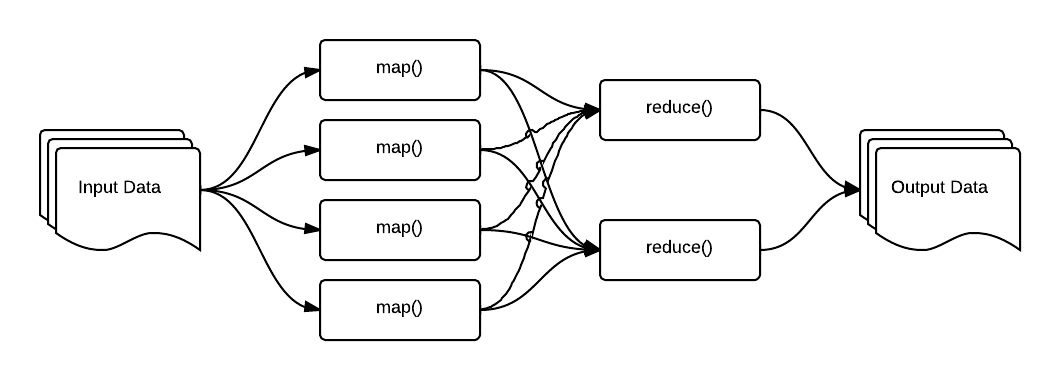
\includegraphics[width=\textwidth]{diagrams/mapreduce.png}
\caption{A simplified explanation of MapReduce}
\label{fig:mapreduce}
\end{figure}

In order to build the Wikipedia traffic data set, we processed a set of raw Wikipedia request logs using Hadoop \cite{hadoop} hosted on Amazon's Elastic Map Reduce \cite{emr} and wrote our job in Python using mrjob \cite{mrjob}, a library originally developed by Yelp for running Python code with Hadoop. For more information, see \Cref{ch:workloads}.

\subsection{CouchDB}
Much of the functionality of ARTS and CRAFTS is built on top of CouchDB \cite{couch}. CouchDB is a document store which allows for the storage of schema-less data in the format of JSON documents. At its core, CouchDB is a powerful key-value store. Storage of documents is primarily based on the specification of an \texttt{id} field which is used to retrieve the document later. CouchDB uses a REST API for all of its operations, so its complete functionality is accessible entirely though HTTP requests.

An important and powerful feature of CouchDB is incremental MapReduce. This functionality behaves in a fashion similar to what was described in the previous section. A user can specify a ``\texttt{view}'' which is a data transformation (\texttt{map}) and optional aggregation (\texttt{reduce}) selectively applied to documents in the database. These views are defined using Javascript or Coffeescript functions which every document is passed through upon insertion to the database as well as during subsequent updates. The results of the view are stored in a B+ tree which allows for quick retrieval of all documents emitted by the view, as well as ranges based on keys.

CouchDB also supports ``\texttt{list}'' functions. Also specified in Javascript, \texttt{list} functions are used to transform documents based up the method by which they are requested. For example, documents requested through a web browser can be transformed into an HTML document for more friendly viewing by end-users.

CRAFTS uses CouchDB as an intermediate store for metric data between itself and external monitoring services. CRAFTS leverages the incremental MapReduce feature to compute aggregates across this data as well. It also uses CouchDB to store intermediate data produced by the analysis pipeline. The web interface to CRAFTS uses \texttt{list} functions in order to transform the data into a format which can be used by the chart library used in the web interface. For more information, see \Cref{ch:datapipe}.